\chapter{Pacemaker+Corosync高可用集群}

高可用集群,是指以减少服务中断时间为目的的服务器集群技术。高可用集群的
出现是为了减少由计算机硬件和软件易错性所带来的损失。它通过保护用户的业
务程序对外不间断提供的服务,把因软件/硬件/人为造成的故障对业务的影响降
低到最小程度。如果某个节点失效,它的备援节点将在数秒钟的时间内接管它的
职责。因此,对于用户而言,集群永远不会停机。高可用集群软件的主要作用就
是实现故障检查和业务切换的自动化。

下面案例是httpd服务的具体实现:

\section{准备工作}

本案例的拓扑图为:

\begin{figure}[!htbp]
  \centering
  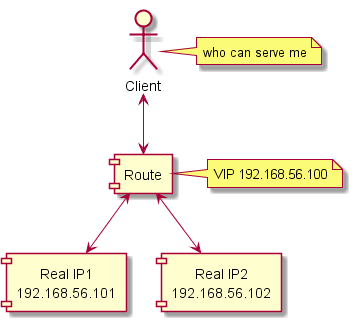
\includegraphics[width=0.5\textwidth]{img/web_topo.png}
  \caption{corosync实验拓扑}
\end{figure}

为了配置一台主机成为HA的节点,通常需要做出如下的准备工作:
\begin{enumerate}[itemsep=0pt,parsep=0pt]
  \item 所有节点的主机名和对应的IP地址解析服务可以正常工作,且每个节点
    的主机名称需要跟“uname -n”命令的结果保持一致;因此,需要保证两个节
    点上的/etc/hosts文件一致;
  \item 两个节点可以基于密钥进行ssh通信;
\end{enumerate}

具体实现为:

\begin{verbatim}
[root@master ~]# cat /etc/hosts
192.168.56.101   master.liucc.com master
192.168.56.102	 slave.liucc.com slave
\end{verbatim}

为了使得重新启动系统后仍能保持如上的主机名称,还需要分别在各节点修改
/etc/sysconfig/network文件。

\begin{verbatim}
master:
# sed -i 's@\(HOSTNAME=\).*@\1master.liucc.com@g'  /etc/sysconfig/network
# hostname master.liucc.com

slave:
# sed -i 's@\(HOSTNAME=\).*@\1slave.liucc.com@g' /etc/sysconfig/network
# hostname slave.liucc.com
\end{verbatim}

各节点生成ssh密钥:

\begin{verbatim}
master:
# cd /root/.ssh
# ssh-keygen -t rsa
# scp id_rsa.pub slave:/root/.ssh/authorized_keys

slave:
# cd /root/.ssh
# ssh-keygen -t rsa
# cat id_rsa.pub >> authorized_keys
# scp authorized_keys master:/root/.ssh
\end{verbatim}

\section{安装软件包}

首先确保已配置本地yum源,然后安装如下依赖包:

\begin{verbatim}
[root@master ~] # yum -y install libibverbs librdmacm lm_sensors \
> libtool-ltdl openhpi-libs openhpi perl-TimeDate
\end{verbatim}

安装完毕依赖包,接下来安装corosync及pacemaker,这里已经准备了相应的软件包,

\begin{verbatim}
[root@master ~]# ls clusterlab
cluster-glue-1.0.6-1.6.el5.i386.rpm       
cluster-glue-libs-1.0.6-1.6.el5.i386.rpm  
corosync-1.2.7-1.1.el5.i386.rpm           
corosynclib-1.2.7-1.1.el5.i386.rpm        
heartbeat-3.0.3-2.3.el5.i386.rpm          
heartbeat-libs-3.0.3-2.3.el5.i386.rpm
libesmtp-1.0.4-5.el5.i386.rpm
pacemaker-1.1.5-1.1.el5.i386.rpm
pacemaker-libs-1.1.5-1.1.el5.i386.rpm
resource-agents-1.0.4-1.1.el5.i386.rpm

[root@master ~]# cd clusterlab
[root@master clusterlab]# yum -y --nogpgcheck localinstall *.rpm
Total size: 17 M
Downloading Packages:
Running rpm_check_debug
Running Transaction Test
Finished Transaction Test
Transaction Test Succeeded
Running Transaction
  Installing     : libesmtp
  Installing     : cluster-glue-libs
  Installing     : corosynclib
  Installing     : cluster-glue
  Installing     : resource-agents 
  Installing     : corosync
  Installing     : heartbeat-libs
  Installing     : pacemaker
  Installing     : pacemaker-libs 
  Installing     : heartbeat
Installed products updated.

Complete!
\end{verbatim}

\section{配置及启动corosync}

下面的配置在master上完成,编辑/etc/corosync/corosync.conf

\begin{verbatim}
[root@master ~]# cd /etc/corosync
[root@master corosync]# cp corosync.conf.example corosync.conf
\end{verbatim}

在文件尾部添加如下内容:

\begin{verbatim}
[root@master corosync]# tail corosync.conf
service {
  ver:  0
  name: pacemaker
}

aisexec {
  user: root
  group:  root
}
\end{verbatim}

并设定此配置文件中 bindnetaddr后面的IP地址为你的网卡所在网络的网络地址,
我们这里的两个节点在192.168.56.0网络,因此这里将其设定为192.168.56.0。
整个配置文件如下:

\begin{verbatim}
[root@master corosync]# cat corosync.conf
# Please read the corosync.conf.5 manual page
compatibility: whitetank

totem {
        version: 2 #版本号
        secauth: off #安全认证
        threads: 0 #线程数,根据CPU个数和核心数确定
        interface {
	        ringnumber: 0 #冗余环号,节点有多个网卡是可定义对应网卡在一个环内
	        bindnetaddr: 192.168.56.0 # 绑定网络地址
	        mcastaddr: 226.94.1.1     # 心跳信息所使用的组播地址
	        mcastport: 5405           # 心跳组播使用的端口
        }
}

logging {
        fileline: off #指定要打印的行
        to_stderr: no #是否发送到标准错误输出
        to_logfile: yes #记录到文件
        to_syslog: yes #记录到syslog
        logfile: /var/log/cluster/corosync.log # corosync日志文件
        debug: off
        timestamp: on #是否打印时间戳,利于定位错误(会消耗CPU资源)
        logger_subsys {
	        subsys: AMF
	        debug: off
        }
}

amf {
        mode: disabled
}

service {
        ver: 0
        name: pacemaker # 定义corosync在启动时自动启动pacemaker
}

aisexec {               # 表示启动corosync的ais功能,以哪个用户身份运行
        user: root
        group: root
}
\end{verbatim}

生成节点间通信时用到的认证密钥文件:

\begin{verbatim}
[root@master corosync]# corosync-keygen
[root@master corosync]# scp -p corosync.conf authkey slave:/etc/corosync

建立corosync日志所需要的目录
[root@master corosync]# mkdir /var/log/cluster
[root@master corosync]# ssh slave "mkdir /var/log/cluster"
\end{verbatim}

接下来就可以启动corosync了,

\begin{verbatim}
[root@master ~]# /etc/init.d/corosync start
Starting Corosync Cluster Engine (corosync):               [  OK  ]
\end{verbatim}

此时,可以查看一下关于corosync引擎是否正常启动的系统日志,

\begin{verbatim}
[root@master corosync]# grep -e "Corosync Cluster Engine" -e "configuration file" /var/log/messages
Feb 28 11:17:02 unionpay smartd[2787]: Opened configuration file /etc/smartd.conf 
Feb 28 11:21:24 master smartd[2770]: Opened configuration file /etc/smartd.conf 
Feb 28 11:44:06 master smartd[2766]: Opened configuration file /etc/smartd.conf 
Feb 28 13:43:05 master corosync[7859]:   [MAIN  ] Corosync Cluster Engine ('1.2.7'): started and ready to provide service.
Feb 28 13:43:05 master corosync[7859]:   [MAIN  ] Successfully read main configuration file '/etc/corosync/corosync.conf'.
\end{verbatim}

查看初始化成员节点通知是否正常发出,
\begin{verbatim}
[root@master corosync]# grep TOTEM /var/log/messages
Feb 28 13:43:05 master corosync[7859]:   [TOTEM ] Initializing transport (UDP/IP).
Feb 28 13:43:05 master corosync[7859]:   [TOTEM ] Initializing transmit/receive security: libtomcrypt SOBER128/SHA1HMAC (mode 0).
Feb 28 13:43:05 master corosync[7859]:   [TOTEM ] The network interface [192.168.56.101] is now up.
Feb 28 13:43:05 master corosync[7859]:   [TOTEM ] A processor joined or left the membership and a new membership was formed.
\end{verbatim}

检查启动过程中是否有错误产生:
\begin{verbatim}
# grep ERROR: /var/log/messages | grep -v unpack_resources
\end{verbatim}

查看pacemaker是否正常启动:
\begin{verbatim}
[root@master corosync]#  grep pcmk_startup /var/log/messages
Feb 28 13:43:05 master corosync[7859]:   [pcmk  ] info: pcmk_startup: CRM: Initialized
Feb 28 13:43:05 master corosync[7859]:   [pcmk  ] Logging: Initialized pcmk_startup
Feb 28 13:43:05 master corosync[7859]:   [pcmk  ] info: pcmk_startup: Maximum core file size is: 4294967295
Feb 28 13:43:05 master corosync[7859]:   [pcmk  ] info: pcmk_startup: Service: 9
Feb 28 13:43:05 master corosync[7859]:   [pcmk  ] info: pcmk_startup: Local hostname: master.liucc.com
\end{verbatim}

如果上面命令执行均没有问题,接着可以执行如下命令启动node2上的corosync
\begin{verbatim}
[root@slave cluster]# ssh slave -- /etc/init.d/corosync start
The authenticity of host 'slave (192.168.56.102)' can't be established.
RSA key fingerprint is 3e:36:02:7a:4c:3c:0d:39:d0:51:a4:86:0f:85:97:c8.
Are you sure you want to continue connecting (yes/no)? yes
Warning: Permanently added 'slave' (RSA) to the list of known hosts.
Starting Corosync Cluster Engine (corosync): [  OK  ]
[root@slave cluster]# ssh slave -- /etc/init.d/corosync status
corosync (pid  10867) is running...
\end{verbatim}

注意:启动node2需要在node1上使用如上命令进行,不要在node2节点上直接启动;

使用如下命令查看集群节点的启动状态:
\begin{verbatim}
[root@master corosync]# crm status
============
Last updated: Sat Feb 28 13:48:11 2015
Stack: openais
Current DC: master.liucc.com - partition with quorum
Version: 1.1.5-1.1.el5-01e86afaaa6d4a8c4836f68df80ababd6ca3902f
2 Nodes configured, 2 expected votes
0 Resources configured.
============

Online: [ master.liucc.com slave.liucc.com ]

\end{verbatim}

从上面的信息可以看出两个节点都已经正常启动,并且集群已经处于正常工作状
态。

由于corosync默认启用了stonith,而当前集群并没有相应的stonith设备,因此
此默认配置目前尚不可用,这可以通过如下命令验正:

\begin{verbatim}
[root@master corosync]# crm_verify -L
crm_verify[7926]: 2015/02/28_13:51:01 ERROR: unpack_resources: Resource start-up disabled since no STONITH resources have been defined
crm_verify[7926]: 2015/02/28_13:51:01 ERROR: unpack_resources: Either configure some or disable STONITH with the stonith-enabled option
crm_verify[7926]: 2015/02/28_13:51:01 ERROR: unpack_resources: NOTE: Clusters with shared data need STONITH to ensure data integrity
Errors found during check: config not valid
  -V may provide more details

\end{verbatim}

我们里可以通过如下命令先禁用stonith:

\begin{verbatim}
[root@master corosync]# crm configure property stonith-enabled=false
\end{verbatim}

使用如下命令查看当前的配置信息:

\begin{verbatim}
[root@master corosync]# crm configure show
node master.liucc.com
node slave.liucc.com
property $id="cib-bootstrap-options" \
	dc-version="1.1.5-1.1.el5-01e86afaaa6d4a8c4836f68df80ababd6ca3902f" \
	cluster-infrastructure="openais" \
	expected-quorum-votes="2" \
	stonith-enabled="false"
\end{verbatim}

从中可以看出stonith已经被禁用。上面的crm,crm\_verify命令是1.0后的版本的
pacemaker提供的基于命令行的集群管理工具;可以在集群中的任何一个节点上执
行。

\section{为集群添加资源}

corosync支持heartbeat,LSB和ocf等类型的资源代理,目前较为常用的类型为
LSB和OCF两类,stonith类专为配置stonith设备而用;可以通过如下命令查看当
前集群系统所支持的类型:

\begin{verbatim}
# crm ra classes 
heartbeat
lsb
ocf / heartbeat pacemaker
stonith
\end{verbatim}

如果想要查看某种类别下的所用资源代理的列表,可以使用类似如下命令实现:

\begin{verbatim}
[root@master ~]# crm ra list lsb
NetworkManager      acpid               anacron             apmd                atd                 auditd              autofs
avahi-daemon        avahi-dnsconfd      bluetooth           capi                conman              corosync            cpuspeed
crond               cups                cups-config-daemon  dnsmasq             dund                firstboot           functions
gpm                 haldaemon           halt                heartbeat           hidd                hplip               httpd
ip6tables           ipmi                iptables            irda                irqbalance          iscsi               iscsid
isdn                kdump               killall             krb524              kudzu               lm_sensors          logd
lvm2-monitor        mcstrans            mdmonitor           mdmpd               messagebus          microcode_ctl       multipathd
mysqld              netconsole          netfs               netplugd            network             nfs                 nfslock
nscd                ntpd                openhpid            openibd             pacemaker           pand                pcscd
portmap             postgresql-9.0      psacct              rawdevices          rdisc               readahead_early     readahead_later
restorecond         rhnsd               rhsmcertd           rpcgssd             rpcidmapd           rpcsvcgssd          saslauthd
sendmail            setroubleshoot      single              smartd              snmpd               snmptrapd           sshd
syslog              sysstat             tomcat              vboxadd             vboxadd-service     vboxadd-x11         vncserver
vsftpd              wdaemon             winbind             wpa_supplicant      xfs                 xinetd              ypbind
yum-updatesd

[root@master ~]# crm ra list ocf heartbeat
AoEtarget           AudibleAlarm        CTDB                ClusterMon          Delay               Dummy               EvmsSCC
Evmsd               Filesystem          ICP                 IPaddr              IPaddr2             IPsrcaddr           IPv6addr
LVM                 LinuxSCSI           MailTo              ManageRAID          ManageVE            Pure-FTPd           Raid1
Route               SAPDatabase         SAPInstance         SendArp             ServeRAID           SphinxSearchDaemon  Squid
Stateful            SysInfo             VIPArip             VirtualDomain       WAS                 WAS6                WinPopup
Xen                 Xinetd              anything            apache              conntrackd          db2                 drbd
eDir88              exportfs            fio                 iSCSILogicalUnit    iSCSITarget         ids                 iscsi
jboss               ldirectord          mysql               mysql-proxy         nfsserver           nginx               oracle
oralsnr             pgsql               pingd               portblock           postfix             proftpd             rsyncd
scsi2reservation    sfex                syslog-ng           tomcat              vmware 

[root@master ~]# crm ra list ocf pacemaker
ClusterMon    Dummy         HealthCPU     HealthSMART   Stateful      SysInfo       SystemHealth  controld      o2cb          ping
pingd      

[root@master ~]# crm ra list stonith
apcmaster               apcmastersnmp           apcsmart                baytech                 bladehpi                cyclades
external/drac5          external/dracmc-telnet  external/hmchttp        external/ibmrsa         external/ibmrsa-telnet  external/ipmi
external/ippower9258    external/kdumpcheck     external/rackpdu        external/riloe          external/sbd            external/vmware
external/xen0           external/xen0-ha        fence_legacy            ibmhmc                  ipmilan                 meatware
nw_rpc100s              rcd_serial              rps10                   suicide                 wti_mpc                 wti_nps
\end{verbatim}

\begin{verbatim}
# crm ra info [class:[provider:]]resource_agent
例如:
[root@master ~]# crm ra info ocf:heartbeat:IPaddr
Manages virtual IPv4 addresses (portable version) (ocf:heartbeat:IPaddr)

This script manages IP alias IP addresses
It can add an IP alias, or remove one.

Parameters (* denotes required, [] the default):

ip* (string): IPv4 address
    The IPv4 address to be configured in dotted quad notation, for example
    "192.168.1.1".

nic (string, [eth0]): Network interface
    The base network interface on which the IP address will be brought
    online.
    
    If left empty, the script will try and determine this from the
    routing table.
    
    Do NOT specify an alias interface in the form eth0:1 or anything here;
    rather, specify the base interface only.
    
    Prerequisite:
    
    There must be at least one static IP address, which is not managed by
    the cluster, assigned to the network interface.
    
    If you can not assign any static IP address on the interface,
    modify this kernel parameter:
    sysctl -w net.ipv4.conf.all.promote_secondaries=1
    (or per device)

cidr_netmask (string): Netmask
    The netmask for the interface in CIDR format. (ie, 24), or in
    dotted quad notation  255.255.255.0).
    
    If unspecified, the script will also try to determine this from the
    routing table.

broadcast (string): Broadcast address
    Broadcast address associated with the IP. If left empty, the script will
    determine this from the netmask.

iflabel (string): Interface label
    You can specify an additional label for your IP address here.

lvs_support (boolean, [false]): Enable support for LVS DR
    Enable support for LVS Direct Routing configurations. In case a IP
    address is stopped, only move it to the loopback device to allow the
    local node to continue to service requests, but no longer advertise it
    on the network.

local_stop_script (string): 
    Script called when the IP is released

local_start_script (string): 
    Script called when the IP is added

ARP_INTERVAL_MS (integer, [500]): milliseconds between gratuitous ARPs
    milliseconds between ARPs

ARP_REPEAT (integer, [10]): repeat count
    How many gratuitous ARPs to send out when bringing up a new address

ARP_BACKGROUND (boolean, [yes]): run in background
    run in background (no longer any reason to do this)

ARP_NETMASK (string, [ffffffffffff]): netmask for ARP
    netmask for ARP - in nonstandard hexadecimal format.

Operations' defaults (advisory minimum):

    start         timeout=20s
    stop          timeout=20s
    monitor       interval=5s timeout=20s
\end{verbatim}

\section{为Web创建IP资源}

接下来要创建的web集群创建一个IP地址资源,以在通过集群提供web服务时使用;
这可以通过如下方式实现:

语法:

\begin{verbatim}
primitive <rsc> [<class>:[<provider>:]]<type>
          [params attr_list]
          [operations id_spec]
            [op op_type [<attribute>=<value>...] ...]

op_type :: start | stop | monitor
\end{verbatim}

例子:

\begin{verbatim}
 primitive apcfence stonith:apcsmart \
          params ttydev=/dev/ttyS0 hostlist="node1 node2" \
          op start timeout=60s \
          op monitor interval=30m timeout=60s
\end{verbatim}


\section{高可用验证}